% UTF-8 encoding
% Compile with latex+dvipdfmx, pdflatex, xelatex or lualatex

\documentclass[hyperref, UTF8]{ctexart}
\usepackage{amssymb}
\usepackage{amsmath}
\usepackage{graphicx}
\usepackage{subfigure}
\usepackage{geometry}
\usepackage{caption}
\usepackage{upgreek}
\newcommand{\under}[1]{\frac{1}{#1}}
\newcommand{\underpone}[1]{\frac{#1}{1+#1}}
\newcommand{\volt}{{\rm V}}
\newcommand{\source}{{\rm S}}
\newcommand{\second}{{\rm s}}
\newcommand{\ampere}{{\rm A}}
\newcommand{\milliampere}{{\rm mA}}
\newcommand{\microampere}{{\rm \upmu A}}
\newcommand{\hertz}{{\rm Hz}}
\newcommand{\ohm}{\Omega}
\newcommand{\kiloohm}{{\rm k}\Omega}
\newcommand{\watt}{{\rm W}}
\newcommand{\kilowatt}{{\rm kW}}
\newcommand{\degree}{^{\circ}}
\newcommand{\farad}{{\rm F}}
\newcommand{\microfarad}{{\rm \upmu F}}
\newcommand{\millifarad}{{\rm mF}}
\newcommand{\henry}{{\rm H}}
\newcommand{\J}{{\rm j}}
\newcommand{\D}{{\rm d}}
\newcommand{\E}{{\rm e}}
\newcommand{\CMRR}{{\rm CMRR}}

\title{电子学基础——第九次作业}
\author{LXQ}
\date{2019.12.05}

\geometry{left=2.0cm, right=2.0cm, top=2.5cm, bottom=2.5cm}
\linespread{1}

\begin{document}

\maketitle

\paragraph{10.51} \label{10.51}
    A student who has a single-ended voltage source constructs the circuit shown in Fig. 10-75, hoping to obtain differential outputs. Assume perfect symmetry but $\lambda = 0$ for simplicity. 

    (b) Viewing $M_1$ as a common-source stage degenerated by the impedance seen at the source of $M_2$, calculate $v_X$ in terms of $v_{in}$.

    (b) Viewing $M_1$ as a source follower and $M_2$ as a common-gate stage, calculate $v_Y$ in terms of $v_{in}$.

    (c) Add the results obtained in (a) and (b) with proper polarities. If the voltage gain is defined as $(v_X - v_Y)/v_{in}$, how does it compare with the gain of differentially driven pairs?

    \begin{figure}[!htb]
        \centering
        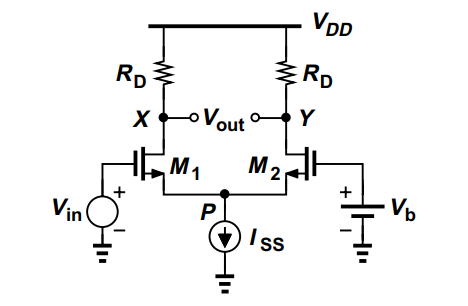
\includegraphics[width=0.312\textwidth]{p10-75.png}
        \caption*{Figure 10-75}
    \end{figure}

\paragraph{解}
    (a) $M_2$从源端看入,输入电阻为$\under{g_{m2}}$,而$M_1$为源简并放大器。则
    $$\frac{v_X}{v_{in}} = -\frac{g_{m1}R_D}{1+g_{m1}\cdot \under{g_{m2}}} = -\frac{g_mR_D}{2}$$

    (b) $M_1$为源极跟随器,则$M_1$源端电压即为$v_{s1}=v_{in}$,而$M_2$为共栅放大器,则
    $$\frac{v_Y}{v_{s1}}=g_{m1}R_D$$
    $$\therefore \frac{v_Y}{v_{in}}=g_{m1}R_D$$

    (c) $$\frac{v_X-v_Y}{v_{in}}=-\frac{3}{2}g_mR_D$$
    这个增益是普通差分放大器增益的1.5倍。

\paragraph{10.70} \label{10.70}
    Compute the common-mode rejection ratio of the stages illustrated in Fig. 10-89 and compare the results. For simplicity, neglect channel-length modulation in $M_1$ and $M_2$ but not in other transistors.

    \begin{figure}[!htb]
        \centering
        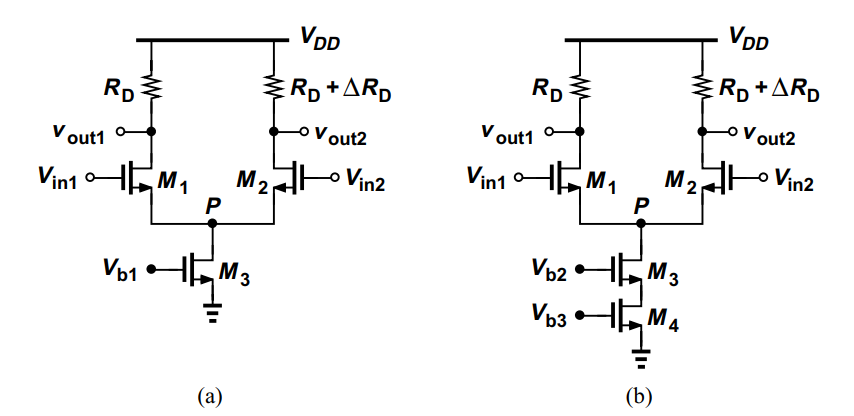
\includegraphics[width=0.569\textwidth]{p10-89.png}
        \caption*{Figure 10-89}
    \end{figure}

\paragraph{解}
    $$\CMRR = 20\log\left|\frac{A_{vd}}{A_{vc}}\right|$$

    (a) 电路对称,可考虑半边电路。由交流小信号电路中$P$为虚地,则
    $$A_{vd}=-g_{m1}R_D$$
    考虑$A_{vc}$时,可将$M_3$视为$r_{o3}$,进而再半边电路中视为$2r_{o3}$,则$M_1$为源简并放大器:
    $$A_{vc}=\frac{-g_{m1}R_D}{1+2g_{m1}r_{o3}}$$
    则
    $$\CMRR = 20\log(1+2g_{m1}r_{o3})$$

    (b) 同(a),$P$再交流小信号电路中仍未虚地,则
    $$A_{vd}=-g_{m1}R_d$$
    再考虑$A_{vc}$,将$M_4$视为$r_{o4}$,则$M_3$为源简并放大器,可视为电阻$r=(1+g_{m3}r_{o3})r_{o4}+r_{o3}$
    从而半边电路中可将其视为$2r=2[(1+g_{m3}r_{o3})r_{o4}+r_{o3}]$
    此时$M_1$仍为源简并放大器:
    $$\therefore A_{vc}=\frac{-g_{m1}R_D}{1+2g_{m1}[(1+g_{m3}r_{o3})r_{o4}+r_{o3}]}$$
    $$\therefore \CMRR = 20 \log [1+2g_{m1}((1+g_{m3}r_{o3})r_{o4}+r_{o3})]$$

\end{document} 